\documentclass{article}
\usepackage{geometry}
 \geometry{
 a4paper,
 total={170mm,270mm},
 left=20mm,
 top=10mm,
 }
\usepackage{graphicx}
\usepackage{listings}
\usepackage{float}
\usepackage{enumitem}
\usepackage{caption}
\usepackage{amsmath}
\usepackage{datetime}
\usepackage{multirow}
\newcommand*{\addheight}[2][.5ex]{%
  \raisebox{0pt}[\dimexpr\height+(#1)\relax]{#2}%
}
\newdate{date}{07}{10}{2016}
\date{\displaydate{date}}
\title{\textbf{Machine Learning - CSCI 5622} \\
HW 4 - Boosting}
\author{\textbf{Santhanakrishnan Ramani}}
\begin{document}
\maketitle

\section*{Analysis}
\begin{enumerate}
\item
Using the AdaBoost code with DecisionTreeClassifier as the base learner to distinguish 4's from 9's,

The Accuracy is \textbf{0.947016460905}\\
The Confusion Matrix is 
\begin{minipage}[b]{0.4\textwidth}
    \begin{tabular}{l r|l l}                      
		& \multicolumn{1}{r|}{} &4   &9   \\ \cline{2-4}
		& \multicolumn{1}{r|}{4} &926   &57  \\
		& \multicolumn{1}{r|}{9} &46   &915  \\ 
	\end{tabular}
\end{minipage} 
\item
The figure below shows the plot of training error and test error vs the number of boosting iterations for different value of depths using Decision Tree Classifier as base with 300 learners.
\begin{table}[h!]
\centering
\begin{tabular}{|c|c|}
	\hline
	\addheight{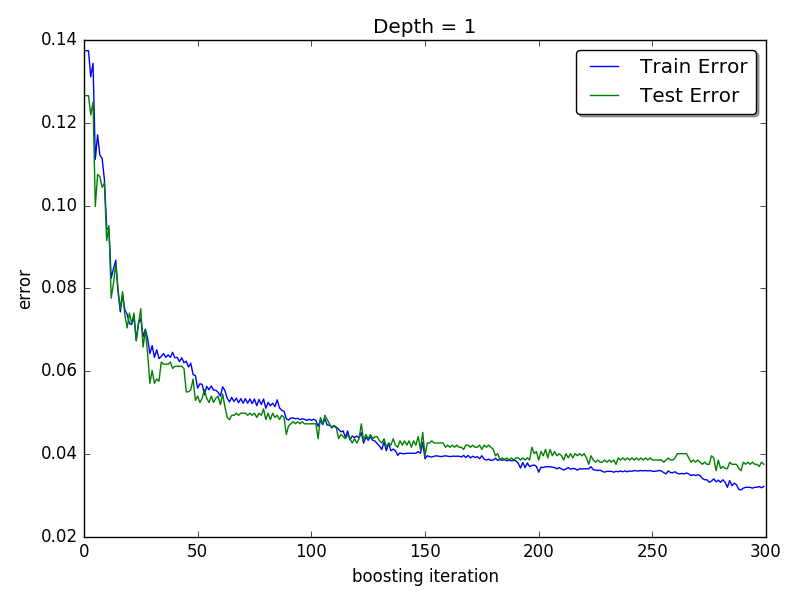
\includegraphics[width=70mm]{images/decision/1.png}} &
	\addheight{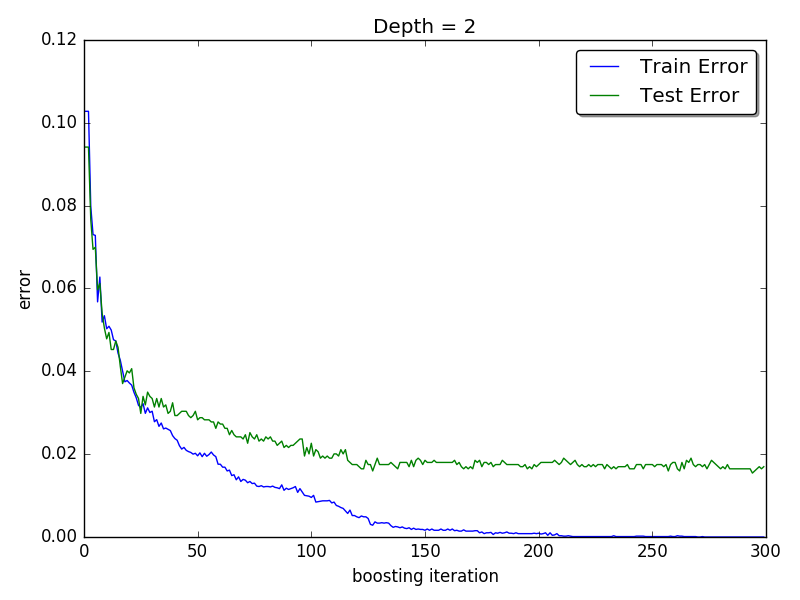
\includegraphics[width=70mm]{images/decision/2.png}} \\  
    \hline 
    \addheight{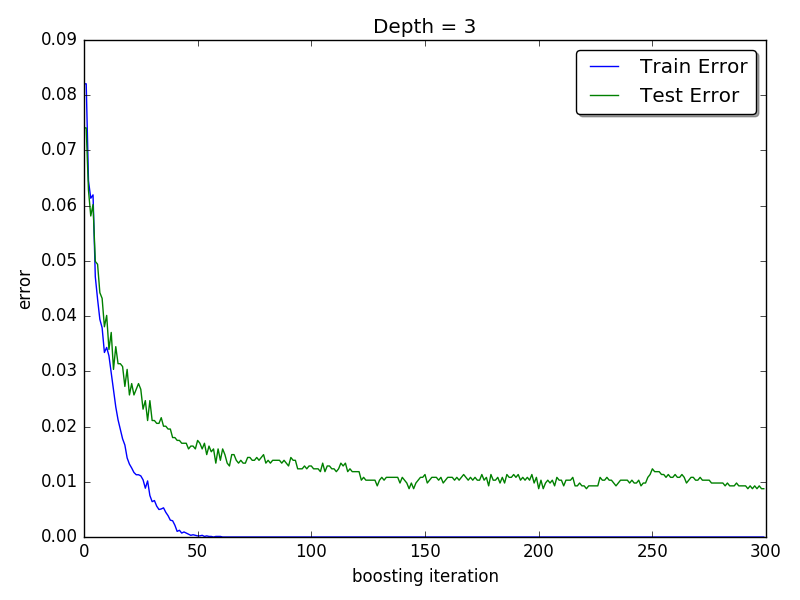
\includegraphics[width=70mm]{images/decision/3.png}} &
	\addheight{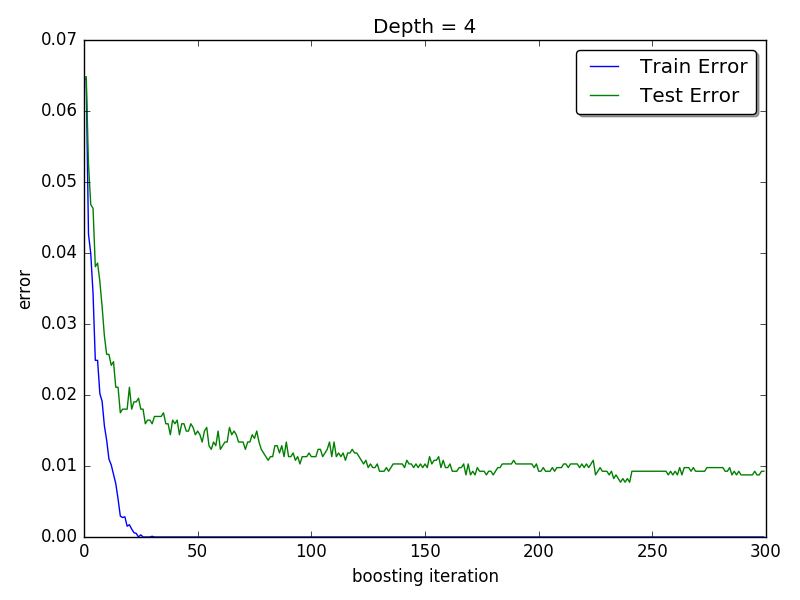
\includegraphics[width=70mm]{images/decision/4.png}} \\  
    \hline 
    \addheight{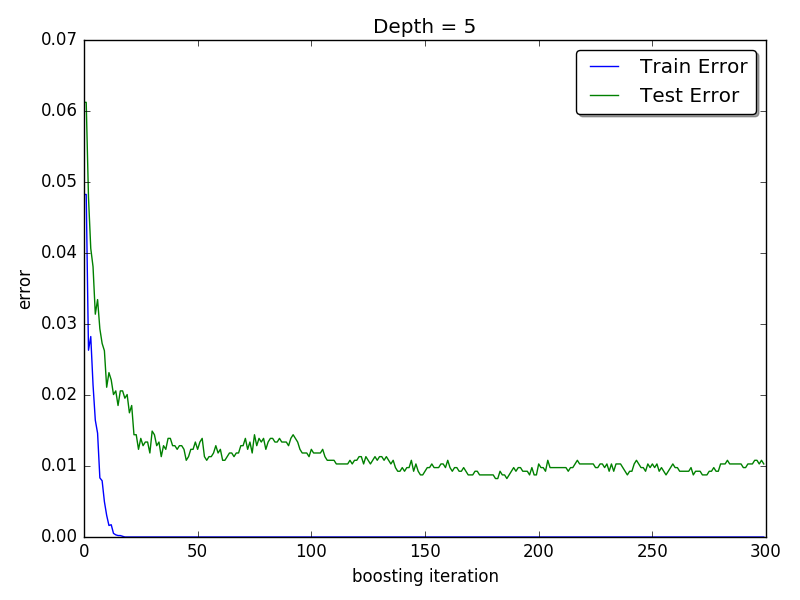
\includegraphics[width=70mm]{images/decision/5.png}} &
	\addheight{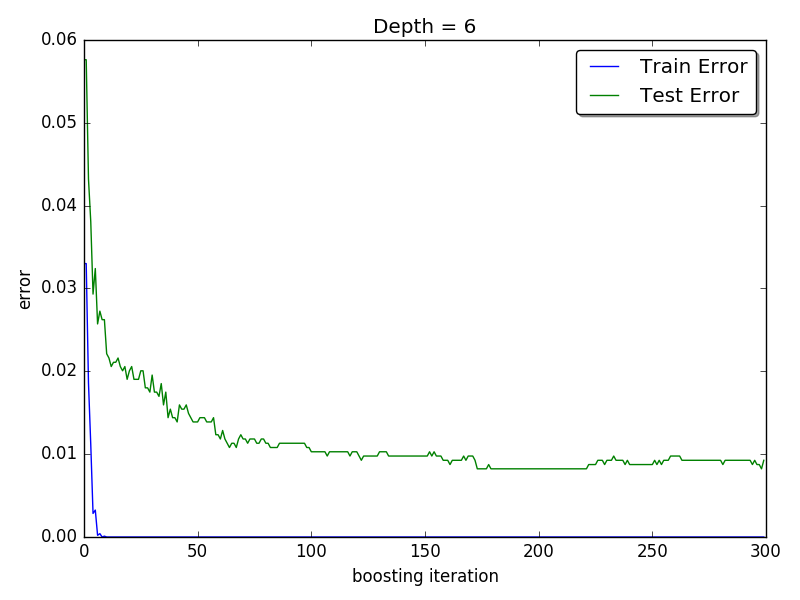
\includegraphics[width=70mm]{images/decision/6.png}}\\  
    \hline 
\end{tabular}
\end{table}

From the figures above, depth equals 3 works the best as the test error is low. We can see that the train error reduces to zero in all classifier after certain iterations and faster as depth increases above 1, and all these classifiers achieve 100\% accuracy on training data. We expect that the test error would go up as a result of over fitting (i.e when the train error is almost zero), but that pattern isn't clearly evident here as it happens very slowly in boosting. Might be if we allow it to run for more than 500 iterations we might be able to see it.
\item
The figure below shows the plot of training error and test error vs the number of boosting iterations for different value of number of iterations using the Perceptron Classifier as base with 200 learners.
\begin{table}[h!]
\centering
\begin{tabular}{|c|c|}
	\hline
	\addheight{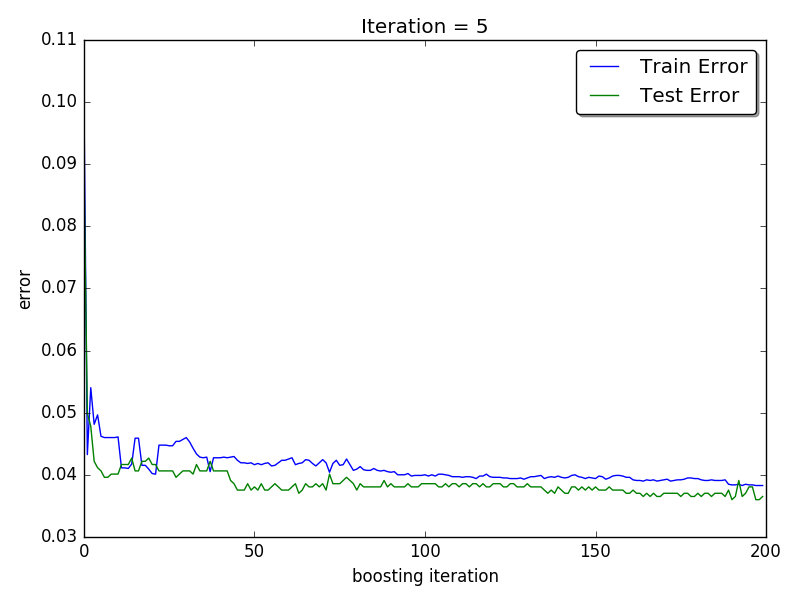
\includegraphics[width=70mm]{images/perceptron/5.png}} &
	\addheight{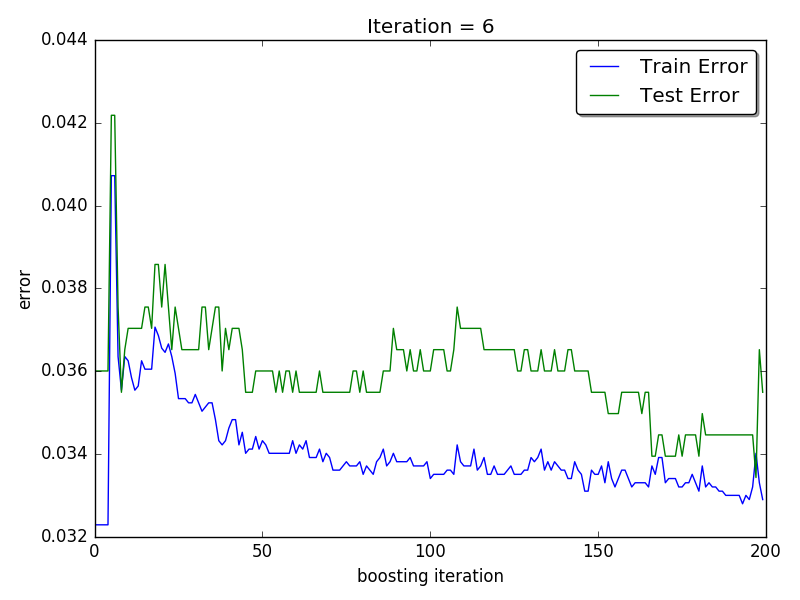
\includegraphics[width=70mm]{images/perceptron/6.png}} \\  
    \hline 
    \addheight{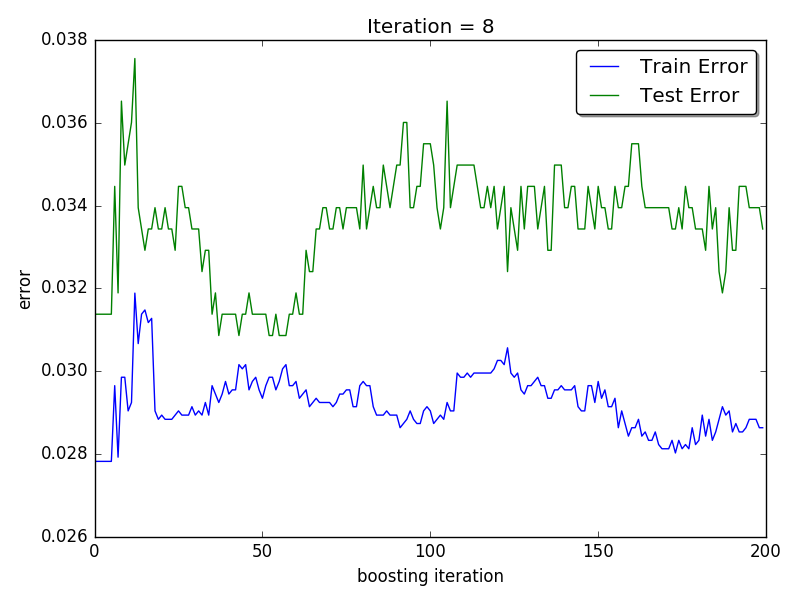
\includegraphics[width=70mm]{images/perceptron/8.png}} &
	\addheight{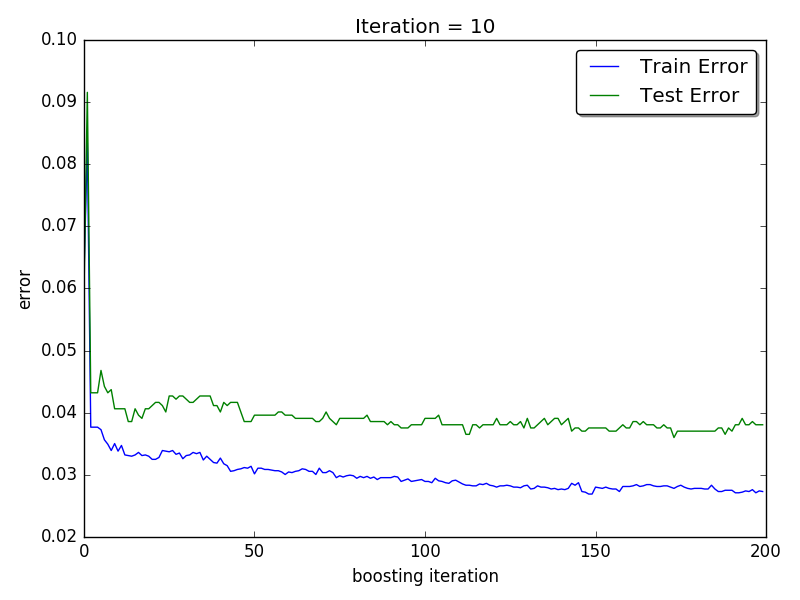
\includegraphics[width=70mm]{images/perceptron/10.png}} \\  
    \hline 
    \addheight{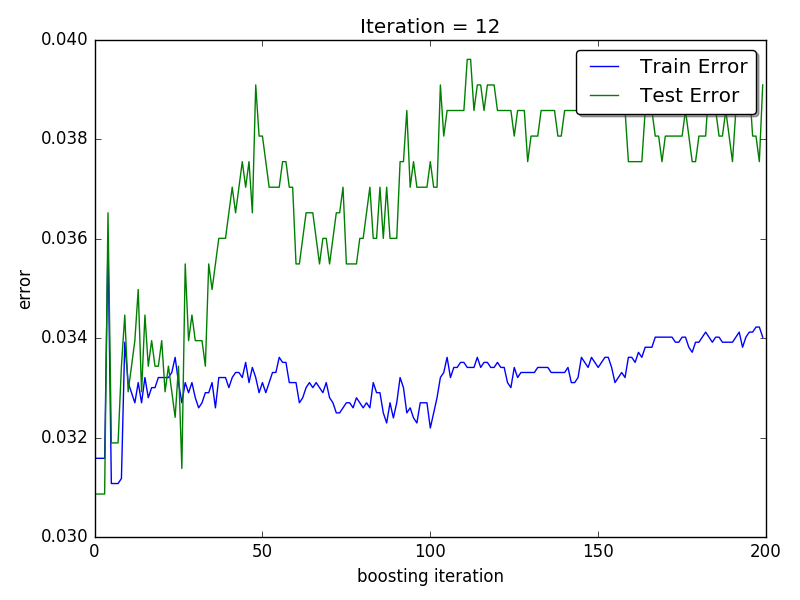
\includegraphics[width=70mm]{images/perceptron/12.png}} &
	\addheight{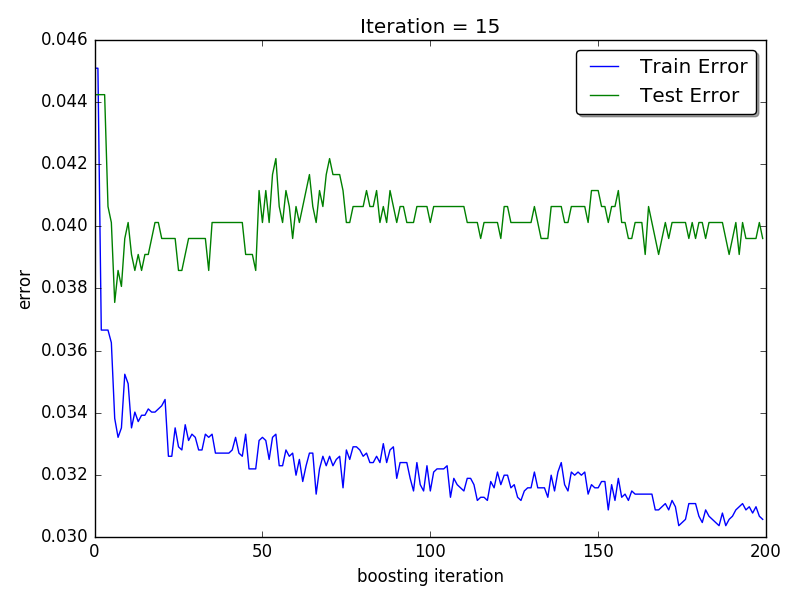
\includegraphics[width=70mm]{images/perceptron/15.png}} \\  
    \hline 
\end{tabular}
\end{table}

From the figures above, we can clearly see that when the number of iterations equals 8, that classifier works the best as the test error is low, and the train error doesn't reduces to zero in all classifier atleast until number of iterations equals 15 and hence doesn't achieve 100\% accuracy on training data. But here we can clearly see that the test error goes up after the number of iterations is greater than 10 and hence predict over fitting.
\end{enumerate}

\end{document}
	